\documentclass[11pt,twoside,a4paper]{book}   %two-page printing
\usepackage[czech, english]{babel}
\usepackage[T1]{fontenc} % pouzije EC fonty
\usepackage[utf8]{inputenc}
\usepackage{graphicx}
%\usepackage{indentfirst} %1. odstavec jako v cestine.


\usepackage{k336_thesis_macros} % specialni makra pro formatovani DP a BP

\newcommand\TypeOfWork{Diplomová práce} \typeout{Diplomova prace}
\newcommand\StudProgram{Elektrotechnika a informatika, strukturovaný, Navazující magisterský}
\newcommand\StudBranch{Výpočetní technika}   % pro prgoram EaI mag. (dobihajici i strukt.)

\renewcommand{\baselinestretch}{1.1}


%Nazev prace, vedouci, autor
\newcommand\WorkTitle{SNMP/XML brána}
\newcommand\FirstandFamilyName{Bc. Tomáš Hroch}
\newcommand\Supervisor{Ing. Peter Macejko}



\begin{document}

\selectlanguage{czech}


\iflanguage{czech}{
	 \typeout{************************************************}
	 \typeout{Zvoleny jazyk: cestina}
	 \typeout{Typ prace: \TypeOfWork}
	 \typeout{Studijni program: \StudProgram}
	 \typeout{Obor: \StudBranch}
	 \typeout{Jmeno: \FirstandFamilyName}
	 \typeout{Nazev prace: \WorkTitle}
	 \typeout{Vedouci prace: \Supervisor}
	 \typeout{***************************************************}
	 \newcommand\Department{Katedra počítačů}
	 \newcommand\Faculty{Fakulta elektrotechnická}
	 \newcommand\University{České vysoké učení technické v Praze}
	 \newcommand\labelSupervisor{Vedoucí práce}
	 \newcommand\labelStudProgram{Studijní program}
	 \newcommand\labelStudBranch{Obor}
}{
	 \typeout{************************************************}
	 \typeout{Language: english}
	 \typeout{Type of Work: \TypeOfWork}
	 \typeout{Study Program: \StudProgram}
	 \typeout{Study Branch: \StudBranch}
	 \typeout{Author: \FirstandFamilyName}
	 \typeout{Title: \WorkTitle}
	 \typeout{Supervisor: \Supervisor}
	 \typeout{***************************************************}
	 \newcommand\Department{Department of Computer Science and Engineering}
	 \newcommand\Faculty{Faculty of Electrical Engineering}
	 \newcommand\University{Czech Technical University in Prague}
	 \newcommand\labelSupervisor{Supervisor}
	 \newcommand\labelStudProgram{Study Programme} 
	 \newcommand\labelStudBranch{Field of Study}
}


\coverpagestarts

%%%%%%%%%%%%%%%%%%%%%%%%%%%    Podekovani / Acknowledgements 

\acknowledgements
\noindent
Na tomto místě bych rád poděkoval vedoucímu práce panu Ing. Peteru Macejkovi za jeho rady a připomínky,
které vedly ke zdárnému dokončení práce. Zároveň můj dík patří i rodině za její podporu.


%%%%%%%%%%%%%%%%%%%%%%%%%%%   Prohlaseni / Declaration 

\declaration{V Praze dne 4.\,5.\,2009}
%\declaration{In Kořenovice nad Bečvárkou on May 15, 2008}


%%%%%%%%%%%%%%%%%%%%%%%%%%%%    Abstract 
 
\abstractpage

The main aim of this project is to develop system, which could connect two communication protocols. The first protocol is
widely used SNMP and the second one is optimized XML-based protocol. The document describes implementation of the system which
includes several optimalizations to reduce memory usage. The program is written in C++ programming language and is designed
for OS Linux.

% Prace v cestine musi krome abstraktu v anglictine obsahovat i
% abstrakt v cestine.
\vglue60mm

\noindent{\Huge \textbf{Abstrakt}}
\vspace{8ex}

\noindent
Cílem tohoto projektu je implementovat systém, jenž by dovoloval spojení dvou komunikačních protokolů. 
Prvním z nich je široce rozšířený protokol SNMP a druhým je navržený optimalizovaný XML protokol. V dokumentu
se kromě samotné implementace programu klade důraz na optimalizace, které snižují nároky na operační paměť. Program
je napsán v jazyce C++, cílový operační systém je Linux. 


%%%%%%%%%%%%%%%%%%%%%%%%%%%%%%%%  Obsah / Table of Contents 

\tableofcontents


%%%%%%%%%%%%%%%%%%%%%%%%%%%%%%%  Seznam obrazku / List of Figures 

\listoffigures


%%%%%%%%%%%%%%%%%%%%%%%%%%%%%%%  Seznam tabulek / List of Tables

\listoftables

\mainbodystarts
% horizontalní mezera mezi dvema odstavci
%\parskip=5pt
%JZ 11.12.2008 parskip bez tolerance? To neni rozumne, myslel jsem, ze sazime v TeXu, ne ve Wordu!
\parskip=5pt plus 4pt minus 4pt
% odstazeni prvniho radku odstavce (neaplikuje se na prvni odstace 
% kapitol, sekci, podsekci atd.)
%\parindent=10pt
%JZ 11.12.2008 -- indent v zavislosti na base font, proc 10pt?
\parindent=1.5em

%nasleduje vstup jednotlivych kapitol
\chapter{Úvod}
Správa velkých počítačových sítí je v dnešní době naprosto samozřejmým úkolem většiny administrátorů. Velké množství spravovaných sítí se neomezuje pouze na lokální prostředí dané firmy či instituce. Může být naopak rozprostřena 
v rámci jednoho města, státu či dokonce několika států najednou. Efektivní spravování takovéto komunikační infrastruktury je úkolem velice náročným.

Jedním z protokolů, který takovouto vzdálenou správu umožňuje, je SNMP. Na jeho základě bylo vybudováno bezpočet aplikací, které mají za úkol sledovat provoz na síti, zatížení určitého systému a v neposlední řadě umožnit administrátorovi
vzdálenou správu daného přepínače, routeru či pracovní stanice.

Protokol SNMP byl navržen v dřívějších dobách a nemusí plně vyhovovat dnešním požadavkům, až už na bezpečnost nebo efektivní využití přenosových médií. Pan Ing. Peter Macejko se ve své diplomové práci (\cite{macejko_dipl}) zaobíral použitím 
technologií XML a návrhu protokolu, který by umožňoval minimálně stejnou funkcionalitu jako protokol SNMP a tento zefektivnil.

Tato práce se zaobírá vytvořením protokolové brány, která by umožnila použít navržený XML protokol ke správě strojů, které stále používají protokol SNMP. Cílem je vytvořit softwarový produkt, který bude plnit úkol prostředníka mezi správcem a spravovaným
strojem. Hlavními problémy jsou implementace navrženého XML protokolu a spojení jej s několika verzemi protokolu SNMP. Důležitým aspektem vývoje je i orientace na snížení nároků na operační paměť. Proto bude v každé části programu kladen důraz na efektivní správu
datových struktur.

V kapitole \ref{kap_snmp} bude podrobně popsán protokol SNMP, jeho komunikační struktury a typy zpráv.

Kapitola \ref{kap_xml} se zabývá rozborem navrženého XML protokolu. 

Analýza systému a diskuse o možných směrech implementace bude popsána v kapitole \ref{kap_navrh_systemu}.

V kapitole \ref{kap_implementace} bude probrána detailní funkčnost implementovaného programu.

Ověření funkce a další testování systému bude popsáno v kapitole \ref{kap_testovani}.


\chapter{SNMP}
\label{kap_snmp}
SNMP, nebo-li Simple Network Management Protocol, je v dnešní době jeden z nejrozšířenějších protokolů na správu počítačové sítě. Je to aplikační protokol, který je součástí TCP/IP rodiny protokolů. 
Byl vyvinut skupinout IETF (Internet Engineering Task Force) a přijat jako standard v roce 1989. Umožňuje sledovat síťový provoz, hledat a řešit problémy, které se při provozu vyskytnou. 

\section{Správní struktura}
SNMP je tvořen sadou standardů, které popisují správu sítě, zahrnující samotný komunikační protokol, definici databázové struktury (SMI) a datové objekty (MIB).

Základním funkčním principem je model Klient - Server (\cite{cisco_snmp}). Struktura spravované sítě se tak dělí na tři klíčové elementy - spravované zařízení, agenta a manažera (viz obrázek \ref{obr_snmp1}).

\begin{figure}[htp]
	\begin{center}
		\includegraphics[width=8cm]{obrazky/02_snmp_principle.png}
		\caption{Základní princip fungování SNMP spravované sítě}
		\label{obr_snmp1}
	\end{center}
\end{figure}

\begin{itemize}
	\item \textbf{Spravovaný systém} - je zařízení (přepínač, router, atd.), na kterém je spuštěn SNMP agent. Toto zařízení shromažďuje sledované informace a pak je
	dává k dispozici manažerovi pomocí SNMP protokolu.
	\item \textbf{Agent} - je software určený pro pro správný překlad požadavků manažera a jejich vykonání na sledovaném systému. Navíc může při sledování posílat manažerovi 
	upozornění, že něco není se systémem v pořádku.
	\item \textbf{Manažer} (NMS - Network Managemet System) - je aplikace, která sleduje a spravuje všechny systémy na sledované síti. Tento systém získává od agentů data, zpracovává je do vizuální podoby, 
	čímž dává možnost administrátorovi mít přehled o celé síti. Zároveň umožňuje měnit sledované parametry přímo u agenta.
\end{itemize}

Komunikace můžeme rozdělit do dvou kategorií dle toho, kdo ji započal. Základní schéma je vyjádřeno na obrázku \ref{obr_snmp2} (\cite{tcpip_snmp}).

\begin{figure}[htp]
	\begin{center}
		\includegraphics[width=12cm]{obrazky/02_snmp_communication.png}
		\caption{Komunikace mezi SNMP manažerem a agentem}
		\label{obr_snmp2}
	\end{center}
\end{figure}

V první části schématu je vyobrazeno standardní chování managera, který posílá dotazy agentovi, který mu odpovídá. Přesný výpis příkazů a zpráv, které si mohou tyto dva systémy mezi sebou vyměňovat, bude 
diskutován dále v této kapitole.

Druhá část schématu popisuje moment, kdy na sledovaném systému nastala nějaká extrémní situace (např. zatížení síťového spoje se blíží k maximu) a agent informuje manažera pomocí zprávy Alert (v SNMP jsou to zprávy
TRAP či INFORM, obě budou diskutovány dále).

Je nutné zmínit, že SNMP protokol pracuje nad transportním protokolem UDP, který je nepotvrzovaný. Není tedy zaručeno, že bude komunikace probíhat bezchybně. Je možné, že některé dotazy a příkazy vůbec nedojdou
ke svému cíli, o čemž se druhá strana nikdy nedozví. Tento fakt může být překážkou při správě rozsáhlých sítí, kde jsou špatné síťové spoje.


\section{SMI, MIB standardy}
Jak již bylo zmíněno dříve, SNMP je sada standardů, která kromě komunikačního protokolu musí definovat i strukturu sledované databáze a samotná data. Tyto informace byly definovány ve standardech SMI a MIB.

\subsection*{SMI}
SMI je zkratkou pro Structure and Identification of Management Information for TCP/IP-based Internets. Tento standard (\cite{rfc1155}) popisuje a definuje základní datové struktury a typy, které protokol využívá.
Jednotlivé objekty jsou pojmenovány a organizovány, aby bylo možno k těmto datům logicky přistupovat. Dle standardu musí mít každý objekt jméno, syntaxi a kódování. Jméno jednoznačně identifikuje objekt. Datový typ
(číslo, řetězec) je určen syntaxí. Kódování zajišťuje správnou serializaci dat při přenosu mezi systémy.

Objekty, identifikovány svým jménem (OID), jsou seřazeny do hierarchické struktury. K identifikaci je použito Abstract Syntax Notation One (ASN.1). Každý OID identifikátor je složen ze skupiny přirozených čísel, které
vyjadřují jeho pozici v pomyslném stromu. Strom má kořen, který je spojen hranami s očíslovanými uzly. Každý uzel může mít vlastní děti, čímž tvoří vlastní podstrom. Takto je možno pokračovat dále do značné hloubky stromu. 
Tento standard též specifikuje, jaké objekty tvoří počátek správní databáze.

\subsection*{MIB}
MIB je zkratka pro Management Information Base. Je to soubor definicí, které popisují parametry a vlastnosti sledovaného zařízení. Existuje více než 100 různých MIB, které popisují různá zařízení. Každý takovýto
soubor definic musí splňovat předpisy SMI, aby byla zaručena správná interpretace objektů. Každý objekt (někdy také nazýván MIB objekt) je unikátně identifikován svým OID a všechny dohromady jsou uspořádány do
stromové struktury tak, jak to bylo popsáno v minulém odstavci. 

Objekty v dané databázi se dělí na \textit{skalární} a \textit{tabelární}. Skalární objekty reprezentují jeden parametr sledovaného zařízení (např. počet ethernetových karet v přepínači), kdežto tabelární objekty
jsou spojením několika spřízněných objektů (např. routovací tabulka je spojením jednotlivých záznamů, coby řádků dané tabulky).

V rámci hierarchického uspořádání jsou vyhrazeny vyšší úrovně stromu (blíže kořenu) jednotlivým standardizujícím organizacím, nižší úrovně jsou poté zadány jednotlivými společnostmi. Každý výrobce si může definovat svojí
privátní větev, do které umístí specifické informace daného zařízení.

MIB, které nebyly standardizovány a oficiálně schváleny, jsou umístěny do větve experimentální.


\section{Verze SNMP protokolu}
Celkem byly doposud standardizovány tři verze protokolu SNMP. Každá z nich definuje svoje specifické datové typy a používané datové rámce pro komunikaci. 

\subsection*{SNMPv1}
V první verzi protokolu byly definovány dvě skupiny datových typů:
\begin{itemize}
	\item Základní datové typy (Simple data types)
	\item Aplikační typy
\end{itemize}

Základní typy jsou definovány v SNMPv1 SMI a definují základní používané hodnoty:
\begin{itemize}
	\item \textbf{INTEGER} - celá čísla od $ -2^{31} $ do $ 2^{31}-1$
	\item \textbf{OCTET STRING}
	\item \textbf{OBJECT IDENTIFIER} - identifikace jednotlivých objektů v rámci normy ASN.1
\end{itemize}

Aplikační specifické typy pak jsou:
\begin{itemize}
	\item \textbf{Network Address} - obecná síťová adresa pro podporu mnoha rodin protokolů
	\item \textbf{IpAddress} - přímo definovaný typ pro IP adresu. SMIv1 podporuje pouze 32 bitovou adresu (IPv4)
	\item \textbf{Counter} - čítač, vyjádřen celým číslem bez znaménka; jeho hodnota se pouze zvyšuje a to až do maxima a pak se vrací zpět na nulu
	\item \textbf{Gauge} - je definována jako nezáporné celé číslo; může hodnotu zvyšovat i snižovat a to v definovaných mezích minima a maxima
	\item \textbf{Time Ticks} - počet hodinových tiků od nějaké události, měřeno v setinách vteřiny
	\item \textbf{Opaque} - typ dovolující přenášet libovolná data v kódování ASN.1. Tato data jsou zakódována jako OCTET STRING a následně přenesena médiem.
	\item \textbf{Integers} - celočíselný typ, který předefinovává specifikaci v SMI
	\item \textbf{Unsigned Integer} - celočíselný typ bez znaménka, který stejně jako předchozí předefinovává specifikaci.
\end{itemize}

Komunikační mechanismus mezi manažerem a agentem je definován pomocí datových rámců, které je možné v rámci SNMPv1 přenášet. Tyto jsou:
\begin{itemize}
	\item \textbf{Get Request} - získání hodnoty uzlu identifikovaného OID (zpráva od manažera agentovi)
	\item \textbf{Get Next Request} - žádost o hodnotu uzlu následujícího po zaslaném OID (od manažera k agentovi)
	\item \textbf{Set Request} - nastavení hodnoty uzlu specifikovaném OID (od manažera k agentovi) 
	\item \textbf{Get Response} - odpověď agenta manažerovi na Get a Set zprávy. Obsahují požadovanou hodnotu
	\item \textbf{Trap} - zpráva od agenta manažerovi, která upozorňuje na nastalé situace na monitorovaném systému.
\end{itemize}

Strukturu jednotlivých SNMP paketů zobrazuje obrázek \ref{obr_snmp3}.

\begin{figure}[htp]
	\begin{center}
		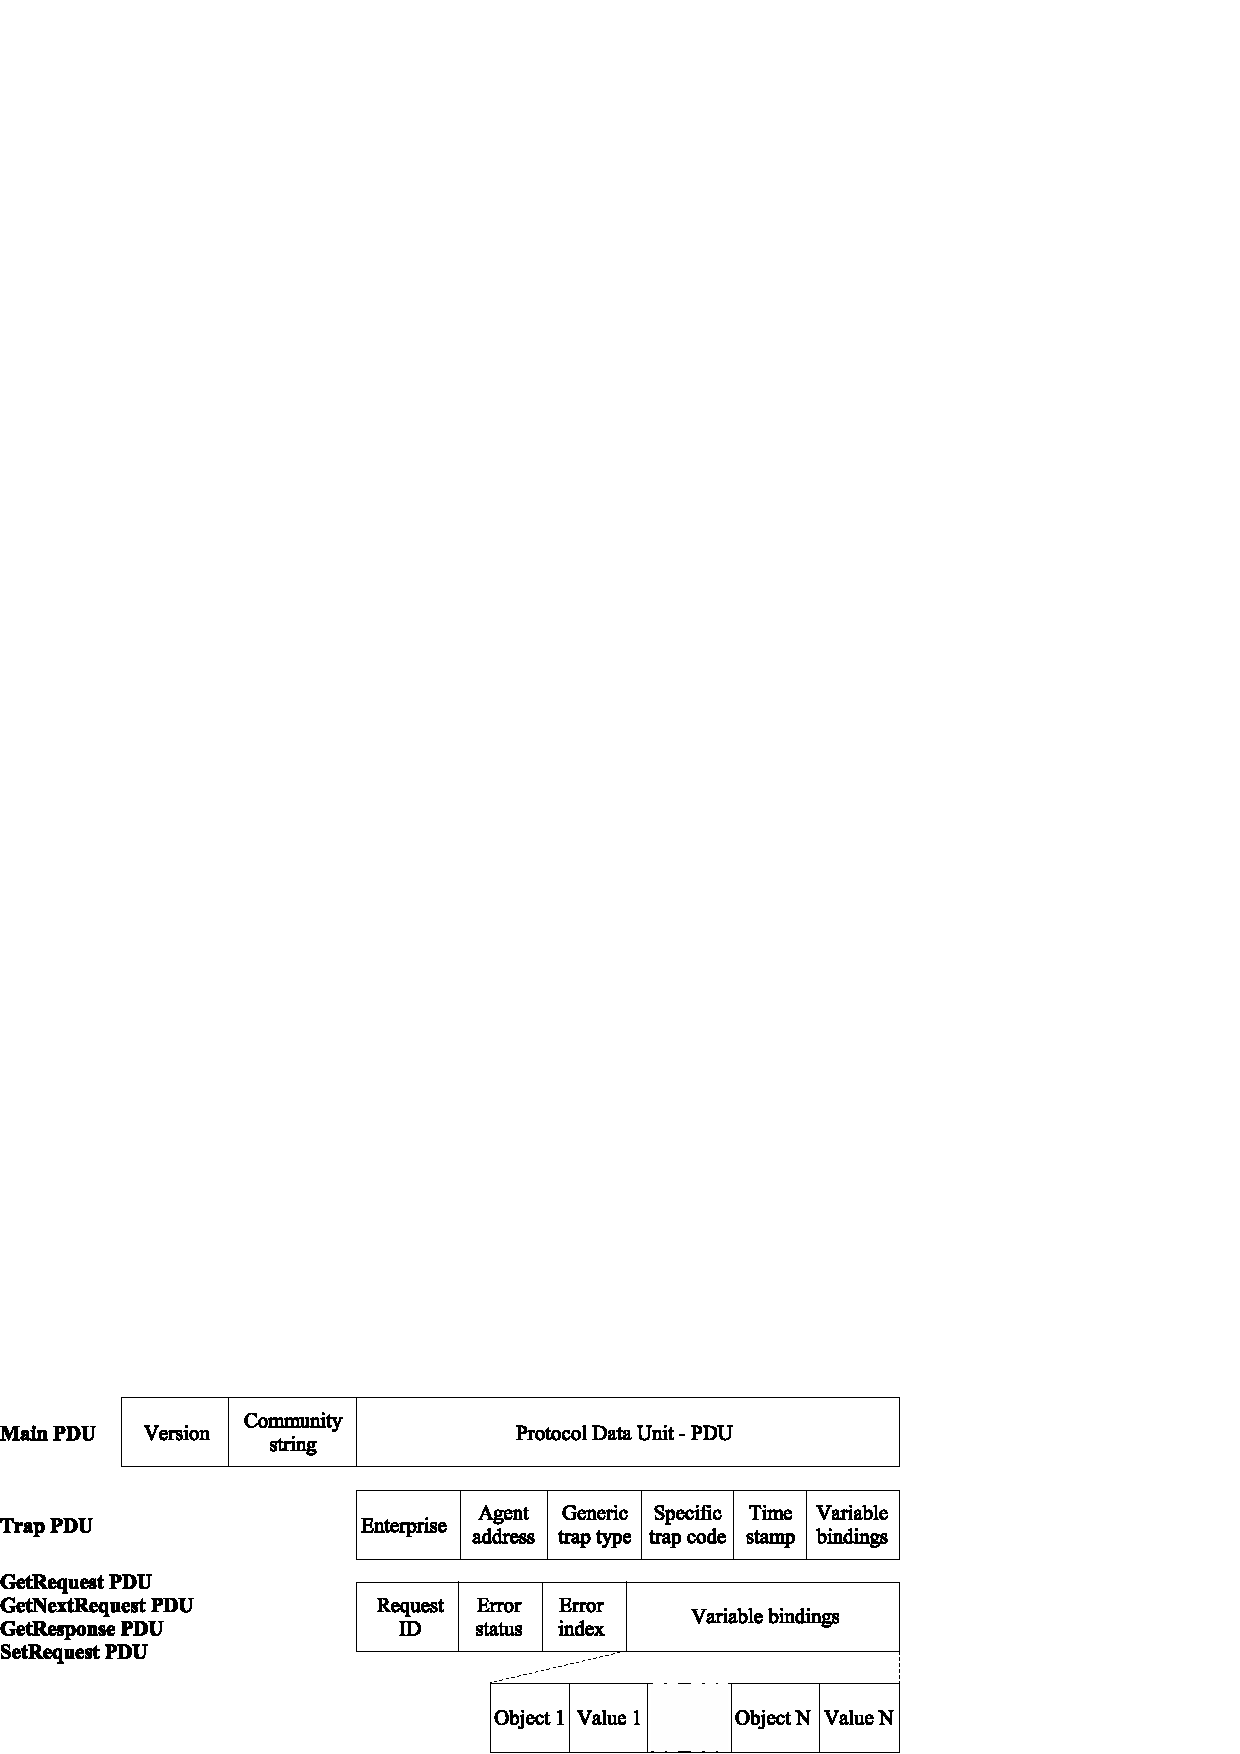
\includegraphics{obrazky/02_snmp_pdu.pdf}
		\caption{Schéma datových paketů protokolu SNMPv1 a v2 (\cite{macejko_dipl})}
		\label{obr_snmp3}
	\end{center}
\end{figure}

Hlavní část datového paketu je tvořena poli Version a Community string. První popisuje verzi SNMP protokolu použitou při komunikaci a druhé je heslo pro přístup
k položkám MIB. Blíže k bezpečnosti v dalším odstavci. Druhá část paketu se liší dle typu zprávy. Paket odeslaný agentem při výskytu monitorované události obsahuje
informace, které popisují druh problému.
\begin{itemize}
	\item \textit{Enterprise} - identifikuje typ zařízení, které zprávu poslalo
	\item \textit{Agent adress} - adresa zařízení, kde běží agent
	\item \textit{Generic trap type} - specifikuje, zda-li se jednalo o některý z předdefinovaných typů událostí (linkDown, linkUp, coldStart, aj.)
	\item \textit{Specific trap type} - identifikuje jednu z mnoha specifických událostí
\end{itemize}

Druhým typem zprávy jsou dotazy a odpovědi, které zasílá manažer a agent na ně odpovídá. Jednotlivá pole mají následující význam:
\begin{itemize}
	\item \textit{Request ID} - pořadové číslo dotazu (aby manažer věděl, na co přišla odpověď)
	\item \textit{Error status} - je nastaven pouze u odpovědi a obsahuje druh problému, který se při dotazu objevil
	\item \textit{Error index} - asociuje problém s instancí objektu.
\end{itemize}

Společným polem pro oba dva typy paketu jsou \textit{Variable bindings} - jsou to dvojice polí, kde jedna část identifikuje objekt a druhá část je jeho hodnota. Například
při dotazu příkazem GET se nastaví název objektu a v odpovědi přijde nastavena i hodnota.

Bezpečnost v této verzi protokolu je založena pouze na takzvaném \textit{community string}u, který vystupuje jako heslo. Existují pouze dvě úrovně zabezpečení
přístupu a to - pouze pro čtení (read only) a čtení-zápis (read-write access). Je patrné, že se používají pouze dvě hesla, každé pro jednu úroveň. Je to velice slabé
zabezpečení, vezmeme-li v úvahu, že toto heslo se posílá nezašifrované a každý, kdo dokáže odchytit jednotlivé pakety, si může tento řetězec přečíst. Tento nedostatek
se pokoušejí odstranit až další verze protokolu.

\subsection*{SNMPv2}
Druhá verze protokolu SNMP byla zaměřena na odstranění nedostatků verze první. Bohužel bylo vydáno několik soupeřících specifikací, označované názvy SNMPv2c, SNMPv2u, SNMPv2*, které
byly vzájemně nekompatibilní. Nicméně zlepšení oproti první verzi bylo několik. Byly definovány nové datové typy, nové zprávy a zlepšená práce s chybami.

Nové datové typy zahrnují rozšíření podpory z 32-bitových čísel na 64-bitová ( Integer32, Integer64, Counter32, ...). 

Přidané zprávy jsou:
\begin{itemize}
	\item \textbf{Get Bulk} - tento operátor se snaží efektivněji využít přenosovou kapacitu kanálu tím, že od agenta si vyžádá sérii informací pomocí jediného dotazu
	\item \textbf{Inform} - stejná funkcionalita jako zpráva Trap ve verzi 1, ale nutné je potvrzení od manažera, že zprávu přijal (Response paket)
	\item \textbf{Response} - odpověď na předcházející Inform zprávu (od manažera k agentovi)
\end{itemize}

Ostatní zprávy SNMPv2 přebírá z předchozí verze a zachovává jejich strukturu. Stejně tak je to i s bezpečností, kde je stále použito heslo ve smyslu community stringu.

\subsection*{SNMPv3}
Třetí verze protokolu SNMP je definována sadou standardů, které nepostihují celkovou funkčnost protokolu jako takového, ale 
dodávají do systému chybějící prvky, hlavně bezpečnosti. Přímo v jednom ze standardů \cite{rfc2570} je řečeno, že tato verze může být chápána jako 
SNMPv2 s dodatečnými administrativními a bezpečnostními schopnostmi.

SNMPv3 definuje tři základní služby:
\begin{itemize}
	\item \textit{Autentifikaci} - datový přenos od manažera k agentovi může být autentifikován, aby se zajistilo ověření identity odesílajícího.
	\item \textit{Soukromí} - šifrování přenášených zpráv.
	\item \textit{Přístupová práva} - agent může definovat přístupová práva, omezovat přístup manažerům pouze k některým akcím a částem dat.
\end{itemize}

Základním principem SNMPv3 je modularita. Každá SNMP entita je tvořena SNMP řídícím systémem a vlastní aplikací. Řídící systém má za úkol 
přijímat, odesílat, šifrovat a dešifrovat všechny zprávy a dále spravuje a kontroluje monitorované objekty. Tyto funkce jsou poté k dispozici jedné či více
aplikací.

Stejně jako předchozí verze, je SNMPv3 založena primárně na transportním protokolu UDP, ale není na něj vázána. Pro přenos dat tak může být použit i jiný protokol.
Vlastní aplikační protokol SNMP je rozdělen do dvou úrovní. První zpracovává datové pakety (PDU processing layer) a druhá zpracovává zprávy (message processing layer).
Nejvyšší úroveň - PDU processing layer - se stará o zpracování příkazů (Get, Get Next, ...), které přijdou v daném paketu. Zpracovaný paket pak předá nižší úrovni - 
message processing layer - která tomuto paketu dodá hlavičku, kde jsou uložena bezpečnostní data.

Na obrázku \ref{obr_snmp4} je vyobrazen formát SNMPv3 zprávy. První část je tvořena systémem zpracování zpráv. Nese informace ohledně verze protokolu, identifikaci zprávy,
maximální délce zprávy a nastavení bezpečnostího modelu. Druhá část je generována bezpečnostním systémem a obsahuje informace o kódování a autorizaci. Třetí část obsahuje samotná 
data.

\begin{figure}[htp]
	\begin{center}
		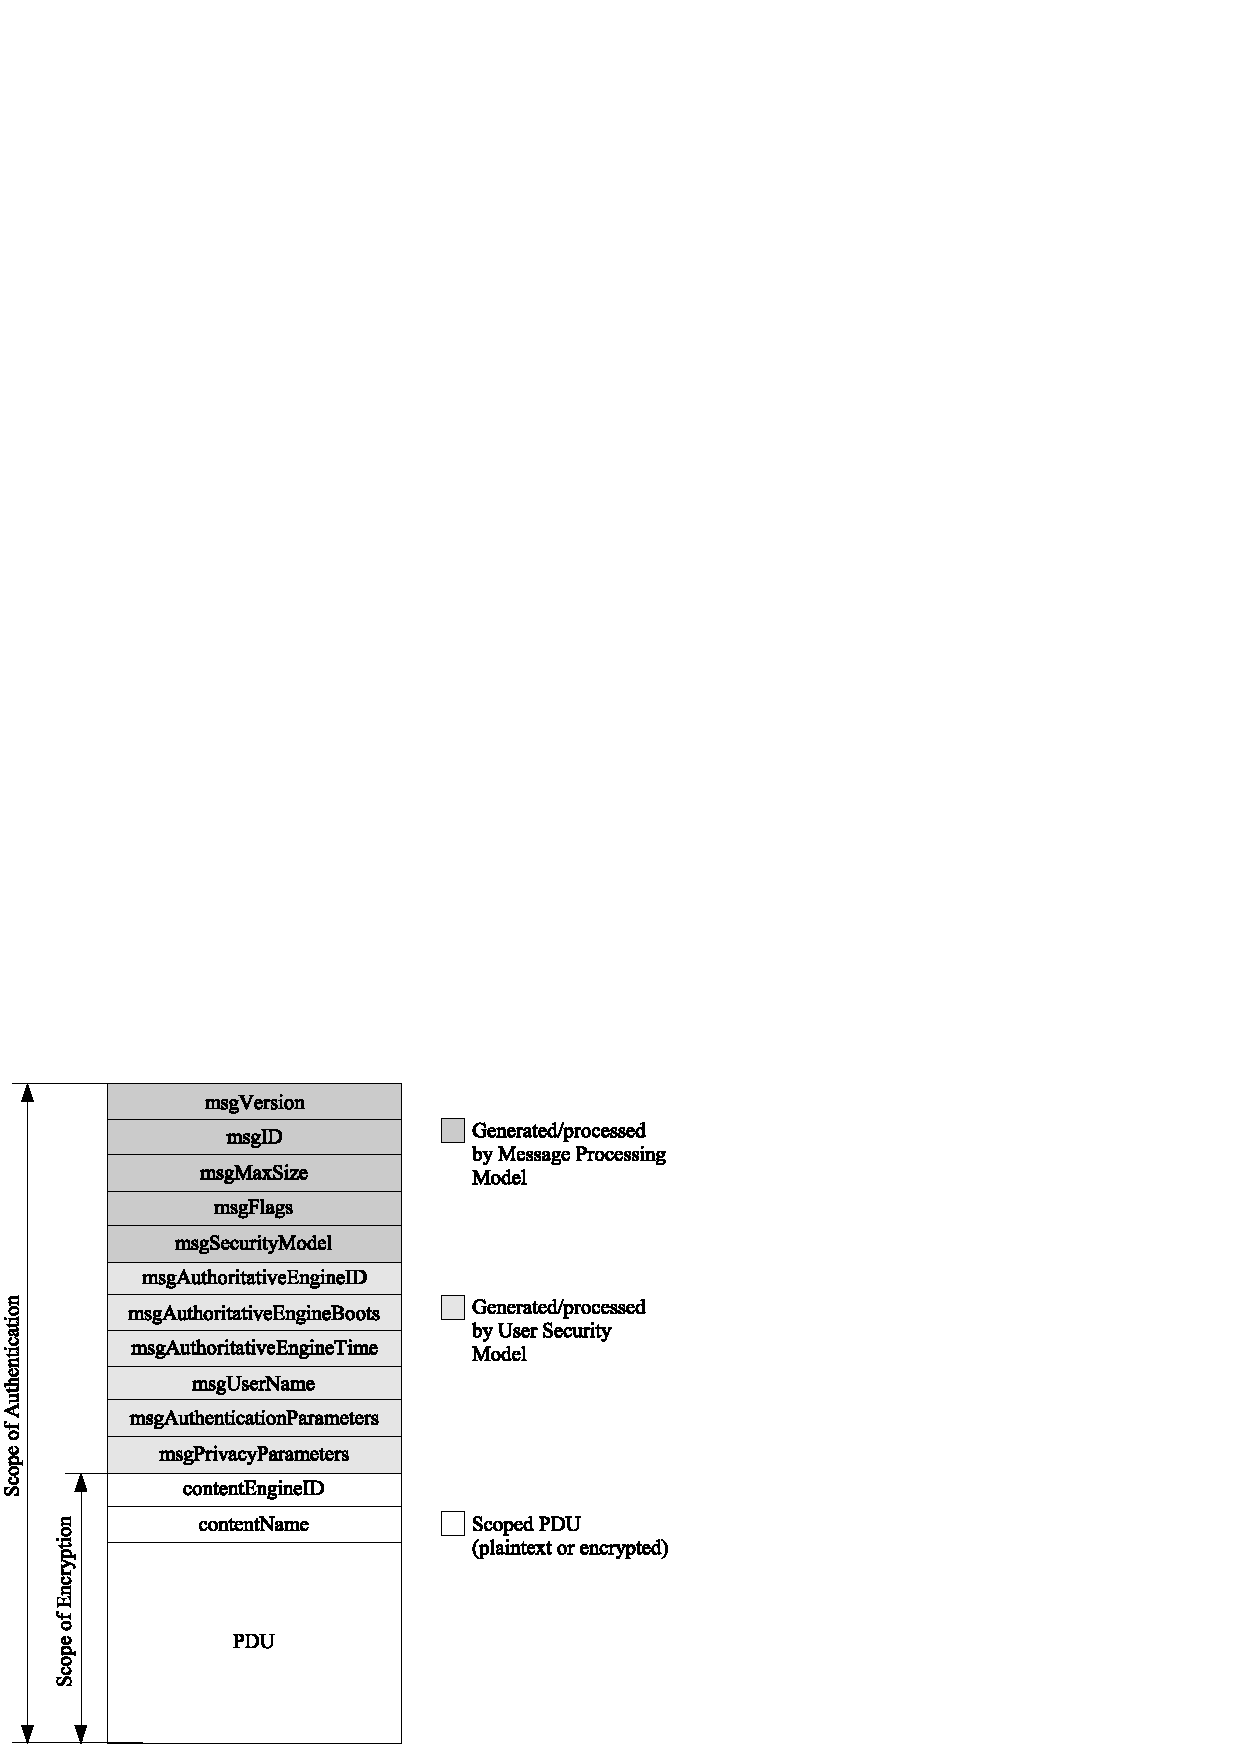
\includegraphics{obrazky/02_snmpv3_pdu.pdf}
		\caption{Schéma datového paketu protokolu SNMPv3 (\cite{macejko_dipl})}
		\label{obr_snmp4}
	\end{center}
\end{figure}


Důležitou součástí nového standardu je i systém přístupových práv (VACM - View-Based Access Control Model). Tento model umožňuje nakonfigurovat agenta tak, 
že specifickému manažerovi bude umožněn přístup pouze k části MIB. Je možné omezit manažera pro přístup pouze k části databáze monitorovaných dat a 
zároveň ještě omezit operace, které nad touto množinou může provádět. Omezení přístupu se provádí pro definované skupiny, kde součástí jedné skupiny může být
více manažerů.


\chapter{XML protokol}
\label{kap_xml}
Pan Ing. Peter Macejko ve své diplomové práci navrh systém vzdálené správy strojů pomocí komunikačního protokolu, využívajícího XML. V této kapitole budou shrnuty všechny 
navržené postupy od mapování SNMP informačního modelu až po komunikační struktury využívané správcem a spravovanými zařízeními.

\section{Obecný informační model}
Informační model je nedílnou součástí celého systému správy dat. Do něj jsou mapována veškerá monitorovaná data a jsou zde i vyjádřeny vztahy mezi daty. Ve skutečnosti
omezuje počet a druh možných dotazů. Výsledný systém, který byl pro popis jednotlivých zařízení navržen vychází z několika různých přístupů abstrakce a popisu dat.

Nejprve byla analýza problému založena na dvou možnostech - přímém mapování MIB stromu do XML dokumentu, kdy by jednotlivé uzly přesně odpovídaly MIB struktuře; objektově
orientovaném využívajícím objektové paradigma. První přístup má výhodu ve snadném převodu MIB databáze do nového formátu, ale naopak ztrácí výhodu snadné rozšiřitelnosti,
která je vlastní XML technolgoii. Problém objektového mapování je nejednoznačné rozmístění uzlů ve stromu na objekty. Takovéto mapování by bylo nutno provádět
neautomatizovaně, tj. s dopomocí člověka.

Výsledkem analýzy problému je systém využívající kousek od obou přístupů. Na nejvyšší úrovni abstrakce je každé zařízení složeno z modulů. Každý model obsahuje jistou
funkcionalitu, která je úplně oddělena od těch zbývajících. Mezi tyto moduly patří i v této práci navrhovaná brána, která propojuje zařízení bez XML podpory s ostatními
částmi sítě. V této chvíli se jedná pouze o obecný návrh každého zařízení.

\subsection{Odvození typů}
Odvozování typů je založeno na principu dědičnosti. Definice jako takové jdou od abstraktního až po detailní popis.

\subsection{Definice modulů}
Jak již bylo řečeno, každé zařízení se skládá z modulů. Jednotlivé moduly jsou též popsány XML schématem. Každé takové schéma
musí splňovat přesné požadavky na poskytované informace.

Musí být detailně popsána funkčnost, přiděleno unikátní jméno, typ a cesta ve stromové struktuře, použitá pro adresaci jednotlivých uzlů. 
SNMP moduly mají definován kořenový element, který je využit pro spojování více MIB informačních bází dohromady.

Přesný popis je možné nalézt v \cite{macejko_dipl} v kapitole 5.2.3.

\subsection{Popis zařízení}
Pro popis zařízení je využito XML schéma, stejně jako pro popis dalších částí (modulů, apod.). Na obrázku \ref{obr_xml_popis_zarizeni} je znázorněno,
jak vypadá zařízení popsané od nejvyšší úrovně. 

\begin{figure}[htp]
	\begin{center}
		\includegraphics[width=15cm]{obrazky/03_popis_zarizeni.png}
		\caption{Popis zařízení v XML schématu (\cite{macejko_dipl})}
		\label{obr_xml_popis_zarizeni}
	\end{center}
\end{figure}

\subsection{Oznamovací zprávy}
Oznámení jsou takové zprávy, které jsou zasílány manažerovi v případě, že se na monitorovaném zařízení vyskytne nějaká událost (shodné s SNMP Trap zprávami).
V rámci SNMP jsou tyto zprávy součástí datového modelu, nicméně tyto specifické uzly MIB stromu nenesou žádná data a jsou tudíž použité pouze při generování typu
chyby či události. 

V navrženém systému jsou všechny možné upozornění (ať již předdefinované, či definované administrátorem) umístěny ve speciálním uzlu stromu \verb|notifications|, 
kde je velice jednoduché dohledat, jaké události mohou způsobit zaslání oznamuvací zprávy. Každý modul pak může mít specifikován speciální typ \verb|NotificationType|,
který popisuje právě onu událost.

\subsection{Adresace dat}
Pro adresaci dat je možno využít postupů XPath a XQuery. Jednotlivými výrazy ať už v jednom či druhém případě se bude manažer dotazovat na jednotlivé uzly v
rámci spravované databáze.


\section{Mapování MIB do XML}
V předchozí části byl rozebrán čistě obecný model popisu zařízení. Pro monitorované stroje, které nejsou kompatibilní s XML protokolem, musí existovat brána,
která bude překládat dotazy z jednoho protokolu na druhý a stejně tak i odpovědi. Je tedy nutné přesně definovat postup přepisu MIB na XML.

Je nutné vyřešit tři základní problémy - jak vyřešit importy jednotlivých MIB do sebe; jak předefinovat datové typy a jak konvertovat celý MIB strom.

\subsection{Importy}
V rámci jednotlivých MIB jsou časté odkazy na báze vyšší úrovně, kdy pak na nižších úrovních definujeme jenom část podstromu. V rámci XML budou definovány 
odkazy jako prostory jmen, které jsou odvozeny od názvu daného MIB. Odkaz na jiné schéma bude proveden použitím odkazů na typ s příslučným názvem prostoru jmen. 

\subsection{Datové typy}
V SNMP, jak bylo řečeno v předchozí kapitole, existuje několik druhů datových typů. Jednoduché (integer, string,...), aplikačně rozšířené (Gauge, IpAddress,...) a 
uživatelem definované.

Jednoduché typy budou mapovány na jejich XML ekvivalent. Na obrázku \ref{obr_xml_smi1_typy} je soupis všech aplikačně rozšířených typů a jejich popis
pomocí XML schématu (v rámci standardu SMIv1).

\begin{figure}[htp]
	\begin{center}
		\includegraphics{obrazky/03_mapovani_smiv1.png}
		\caption{Mapování aplikačních typů SMIv1 do XML schématu (\cite{macejko_dipl})}
		\label{obr_xml_smi1_typy}
	\end{center}
\end{figure}

\begin{table}
	\centering
	{\footnotesize
	  \begin{tabular}{|p{15cm}|}
      \hline
\begin{verbatim}...
    <xsd:element name="NodeName" type="MIBName:NodeNameType"/>
...
<xsd:simpleType name="NodeNameType">
  <xsd:annotation>
    <xsd:documentation xml:lang="en">DescrText</xsd:documentation>
    <xsd:appinfo>
      <status>StatusType</status>
      <access>AccessType</access>
      <oid>AbsoluteOID</oid>
    </xsd:appinfo>
  </xsd:annotation>
  <xsd:restriction base="NodeType"/>
</xsd:simpleType>\end{verbatim}\\
      \hline
    \end{tabular}
  }
	\caption{Mapování makra OBJECT-TYPE, jednoduchý typ (SMIv1) (\cite{macejko_dipl})}
	\label{tab_xml_smi1_simple_type}
\end{table}

Součástí SMI je i možnost definovat vlastní typy. I pro tyto případy je nutno uvést definici překladu. Existují tři základní omezení při vytváření vlastních typů -
výčet, délka řetězce a rozmezí hodnot. Všechny tyto typy jsou detailně popsány a vyobrazeny v \cite{macejko_dipl}, kapitola 5.3.1.

\subsection{MIB strom}
Navržený systém využívá při mapování celého stromu oddělení definicí typů od samotné struktury stromu. Typy jsou definovány globálně a zároveň separátně od 
struktury a to z důvodu možného použití typů v rámci jiného modulu a zároveň při omezení přístupových práv do danéh oblasti stromu. V MIB jsou objekty
definovány makry (specifikované v SMI), které popisují několik základních typů uzlů. SMIv1 specifikuje OBJECT-TYPE a TRAP-TYPE makra.

OBJECT-TYPE makro definuje uzel, který obsahuje nějaká data. Může to být samotná hodnota, položka, nebo celá řádka tabulky. Mapování pak závisí na
položce \verb|SyntaxType| v samotné definici makra.

Pakliže je hodnota položky základním, rozšířeným či uživatelsky definovaným typem, bude vytvořena globální definice typu a položka bude tvořena elementem
s jednoduchým typem. Schematicky vyjádřeno v tabulce \ref{tab_xml_smi1_simple_type}.

Jestli bude hodnotou \verb|SEQUENCE|, bude vytvořen "řádkový" typ (tabulka \ref{tab_xml_smi1_sequence}).

Hodnota \verb|SEQUENCE OF| pak vyjadřuje množinu řádkových typů (tabulka \ref{tab_xml_smi1_sequenceof}).


\begin{table}
	\centering
	{\footnotesize
	  \begin{tabular}{|p{15cm}|}
      \hline
\begin{verbatim}...
    <xsd:element minOccurs="0" maxOccurs="unbounded"
             name="NodeName" type="MIBName:NodeNameType"/>
...
<xsd:complexType name="NodeNameType">
  <xsd:sequence>
    <xsd:element name="..child.." type="..childType.."/>
    ...
  </xsd:sequence>
</xsd:complexType>\end{verbatim}\\
      \hline
    \end{tabular}
  }
	\caption{Mapování SEQUENCE, makro OBJECT-TYPE (\cite{macejko_dipl})}
	\label{tab_xml_smi1_sequence}
\end{table}

\begin{table}
	\centering
	{\footnotesize
	  \begin{tabular}{|p{15cm}|}
      \hline
\begin{verbatim}...
  <xsd:element name="atTable">
    <xsd:complexType>
      <xsd:sequence>
        <xsd:element ..SEQUENCE.. />
      </xsd:sequence>
    </xsd:complexType>
  </xsd:element>
...\end{verbatim}\\
      \hline
    \end{tabular}
  }
	\caption{Mapování SEQUENCE OF, makro OBJECT-TYPE (\cite{macejko_dipl})}
	\label{tab_xml_smi1_sequenceof}
\end{table}

Dalším typem objektu jsou upozornění definované pomocí TRAP-TYPE makra. Tyto definují uzly bez hodnot, pouze specifikují danou událost. V navrženém systému
tedy nemusí být součástí stromu, ale pouze globálních typových definicí. Bude použit jednoduchý typ popisující čas a den (datetime type) se speciálním elementem
v části \verb|appinfo|.

\begin{table}
	\centering
	{\footnotesize
	  \begin{tabular}{|p{15cm}|}
      \hline
\begin{verbatim}<xsd:simpleType name="NodeNameType">
  <xsd:annotation>
    <xsd:documentation xml:lang="en">DescrText</xsd:documentation>
    <xsd:appinfo>
      <enterprise>EnterpriseName</enterprise>
      <variable>VariableType</variable>
      <reference>ReferenceType</reference>
      <trapNumber>TrapNumber</trapNumber>
    </xsd:appinfo>
  </xsd:annotation>
  <xsd:restriction base="xsd:dateTime"/>
</xsd:simpleType>\end{verbatim}\\
      \hline
    \end{tabular}
  }
	\caption{Mapování TRAP-TYPE makra (\cite{macejko_dipl})}
	\label{tab_xml_trap_type}
\end{table}

\newpage

\section{Zprávy}
Navrhovaný systém by měl využívat spolehlivého a potvrzovaného přenosového protokolu, na rozdíl od nepotvrzovaného SNMP. Zaroveň by mělo být možno
přenášet zprávy v co nejjednodušším formátu. Proto bylo rozhodnuto o použití protokolu HTTP, který využívá přenosový protokol TCP, čímž je zajištěn 
splehlivý přenos. Všecha data se budou přenášet pomocí HTTP zprávy POST.

HTTP je bezestavový protokol. Veškerá komunikace se sestává z dvojice dotaz a odpověď. Na serveru se neudržují jakékoliv další informace ohledně probíhajícím
spojení. Tato nenáročnost dovoluje implementaci na velice různorodém hardwaru.

Bezpečnost přenosu může být řešena za použití tunelování paketů (IPSec, STunel,...), nebo je možno využít výhody HTTPS (HTTP over SSL). 

Veškerá přenášená data budou ve formátu XML dokumentu s kořenovým uzlem \verb|message|. Tento uzel má několik atributů, které specifikují jeho zpracování a přístupová
práva. Jsou to \verb|queue|, \verb|password|, \verb|context|. První atribut určuje frontu (může být založeno na prioritním zpracování), ve které bude požadavek zpracován.
V principu ale nejsou agenti ani brány povinni takovouto funkčnost implementovat. Zprávy pak budou zpracovány sekvenčně a odpovědi budou generovány v přesném pořadí tak, 
jak přišly dotazy. Zbylé dva atributy slouží pro vymezení přístupu uživatele (\verb|context|) na určitý podstrom dat. 

Bylo již naznačeno, že zpráva může obsahovat několik jednotlivých dotazů. Struktura zprávy je vyjádřena na obrázku \ref{obr_xml_struktura_zpravy}.

\begin{figure}[htp]
	\begin{center}
		\includegraphics{obrazky/03_struktura_zpravy.png}
		\caption{Struktura XML zprávy}
		\label{obr_xml_struktura_zpravy}
	\end{center}
\end{figure}

Dotazy a odpovědi, které definují komunikaci mezi manažerem a klientem, jsou popsány níže. Přesné XML schéma definující úplnou strukturu zpráv obsahuje (\cite{macejko_dipl}, příloha D).

\subsubsection*{DISCOVERY}
Tato zpráva je první, kterou zašle manažer agentovi, aby zjistil, jaká monitorovaná data jsou k dispozici.
Povinným atributem je číslo verze protokolu (\verb|protocolVersion|) a nepovinným je \verb|fullDescription| pro bližší specifikace
typů spravovaných dat.

\begin{verbatim}
<message context="honza">
  <discovery protocolVersion="1.0" msgid="123" />
</message>
\end{verbatim}

\subsubsection*{PUBLICATION}
Agentova odpověď na manažerův dotaz DISCOVERY. V rámci zprávy je uvedeno, jakou verzi protokolu agent používá a jaká data spravuje. Tato data jsou pak
manažerem zpracována a použita jako informační model.

\begin{verbatim}
<publication msgid="123">
  <info>
    <xpath>1.0</xpath>
    ...
  </info>
  <dataModel>
    ... XML schema popisující spravovaná data ...
  </dataModel>
</publication>
\end{verbatim}

Pakliže agent nepodporuje danou verzi protokolu, musí odpovědět chybovou zprávou:

\begin{verbatim}
<publication msgid="123">
  <error code="1">Protocol not supported</error>
</publication>
\end{verbatim}

\subsubsection*{GET}
Tímto dotazem se manažer ptá agenta na hodnotu nějakého uzlu. Pro specifikaci jakého je nutno použít XPath či XQuery.

\begin{verbatim}
<get msgid="123">
  <xpath>
    device/data/interface
  </xpath>
</get>
\end{verbatim}


\subsubsection*{SET}
Zpráva SET je určena pro nastavení hodnoty uzlu. Struktura je podobná zprávě GET, ale obsahuje navíc element \verb|value|.

\begin{verbatim}
<set msgid="123">
  <xpath>
    device/data/interface/status
  </xpath>
  <value>4</value>
</set>
\end{verbatim}

\subsubsection*{RESPONSE}
Odpověď na zprávy GET a SET. V případě GET nese zpráva příslušná data. Pakliže je to odpověď na SET, je to pouze potvrzení, že hodnota byla uzlu úspěšně nastavena.

\begin{verbatim}
<response msgid="123">
  <value>4</value>
</response>

<response msgid="123" />
\end{verbatim}

\subsubsection*{EVENT}
Pro oznamování asynchronních událostí, je tu zpráva EVEN (stejná funkcionalita jako TRAP u SNMP). Přenášené informace specifikují, která událost vyvolala toto oznámení,
kdo to poslal, datum a čas, případně nějaká další data, která by mohla být při řešení problému užitečná.

\begin{verbatim}
<event msgid="123" timestamp="" senderID="router1" eventSpec="/device/notifications/dhcp/noFreeLease">
  <data>
    <value valueLocation="/data/services/dhcp/leases/free">0</value>
    <value valueLocation="/data/services/dhcp/leases/used">50</value>
  </data>
</event>
\end{verbatim}

Je nutné, aby doručení této zprávy bylo potvrzeno. Což bude dodrženo použitým protokolem.

\subsubsection*{SUBSCRIBE}
Touto zprávou se manažer přihlásí k opakovanému zasílání dat. Potvrzením je pak první doručení dat - zpráva DISTRIBUTION - nebo chybové zprávy, že je něco v nepořádku.
Je možné specifikovat ještě nepovinný atribut \verb|frequency| - doba ve vteřinách, po které mají být opakovaně zasílány zprávy. Další nepovinné atributy \verb|distrid| a \verb|delete|
jsou využity pro editaci či smazání daného přihlášení.

\begin{verbatim}
<subscribe msgid="123" frequency="150">
  <xpath>/device/data/interface/status</xpath>
</subscribe>
\end{verbatim}

\subsubsection*{DISTRIBUTION}
Zpráva obsahuje data, o která si manažer řekl. Je nutné, aby odesílaná data byla ve stejném pořadí, ve kterém byla ve zprávě SUBSCRIBE. 
Povinný atribut \verb|distrid| je určený k identifikaci příchozích dat u manažera.

\begin{verbatim}
<distribution msgid="123" distrid="5678">
  <value>1</value>
  <valuea>500</value>
</distribution>
\end{verbatim}

Příjem těchto dat je též nutné potvrdit, což zajistí transportní protokol.




\chapter{Návrh systému}
\label{kap_navrh_systemu}
V předchozích dvou kapitolách byla rozebrána teoretická část problému. V této kapitole shrneme požadavky vyplývající z teorie, které je nutno zakomponovat do
výsledného systému. Nejprve bude schématicky vyjádřena obecná funkcionalita systému, která se následně bude rozebírat detailněji.

\section{Teoretické požadavky}
Nároky na systém, které vyplývají z teorie můžeme rozdělit do třech částí - implementace SNMP protokolu, implementace navrženého XML protokolu a propojení těchto dvou protokolů dohromady.

Hlavním požadavkem, který vyplývá i ze zadání práce, je vytvořit modulární systém, který bude nejenom spojovat současné verze protokolů, ale bude počítat i s potenciálním rozšířením do
budoucna. Obecné schéma navrhovaného systému zobrazuje obrázek \ref{obr_an_obecne_schema}. 

\begin{figure}[htp]
	\begin{center}
		\includegraphics[width=15cm]{obrazky/04_obecne_schema.png}
		\caption{Schéma navrhovahého systému}
		\label{obr_an_obecne_schema}
	\end{center}
\end{figure}

Zde je vidět, že oba dva protokolové moduly jsou na sobě nezávislé a jejich interakce spočívá v předávání si zpráv. Nyní přejděme k detailnějším požadavkům na výše zmíněné části systému.

V rámci \textit{SNMP protokolu} je požadováno
\begin{itemize}
	\item implementace komunikačních struktur protokolů SNMPv1 a SNMPv2
	\item převzetí bezpečnostního schématu z tohoto protokolu
\end{itemize}

\textit{XML orientovaná část programu } má za úkol
\begin{itemize}
	\item implementovat komunikační struktury navrženého protokolu
	\item navrhnout efektivní správu XML struktur v paměti
	\item poskytnout XML manažerům transparentní získání dat z monitorovaných zařízení
	\item mapovat rozšířenou množinu funkcí v rámci XML protokolu do SNMP
	\item s manažery komunikovat pouze přes HTTP/HTTPS protokol
\end{itemize}
Spojením protokolů je myšlen přechod od databázových struktur jednoho protokolu k druhému. V našem případě je to transformace SNMP MIB do XML, jak bylo vysvětleno v kapitole \ref{kap_xml}.

\subsection{XML}
Nejprve se zaměříme na reprezentaci dat, které budou v rámci XML popisovat jak bránu, tak monitorované zařízení. Z předchozích kapitol vyplynulo, že bude použito částečně objektového přístupu a přímého mapování MIB.
Strukturu dat bude popisovat XML dokument, strom, který má strukturu vyjádřenou na obrázku \ref{obr_an_strom_struktura}.

\begin{figure}[htp]
	\begin{center}
		\includegraphics{obrazky/04_schema_dokumentu.png}
		\caption{Obecná struktura XML dokumentu}
		\label{obr_an_strom_struktura}
	\end{center}
\end{figure}

Kořenový uzel specifikuje celé zařízení vystupující jako protokolová brána, obsahuje tyto elementy:
\begin{itemize}
	\item \textbf{info} - tento element obsahuje text, kterým je popsáno dané zařízení.
	\item \textbf{services} - element vymezující poskytované služby (při širší implementaci může obsahovat služby DNS, DHCP, apod.)
	\item \textbf{xmlbnmGate} - naše služba poskytující spojení XML a SNMP protokolu
	\item \textbf{device} - je podelementem \textbf{xmlbnmGate} a vymezuje jedno monitorované zařízení
\end{itemize}

Prvky \textbf{device} jsou do XML dokumentu přidávány na základě informací v konfiguračním souboru (viz kapitola \ref{sec_an_struktura_programu}).

Strukturu elementu \textbf{device} popisuje obrázek \ref{obr_an_device_struktura}. Každý takovýto element bude obsahovat následující informace:
\begin{itemize}
	\item \textbf{info} - stejně jako kořenový element popisuje dané zařízení
	\item \textbf{notifications} - obsahuje elementy a typy upozornění (TRAP zprávy v rámci SNMP), na které manažer čeká
	\item \textbf{subscriptions} - obsahuje informace o datech, které si nechává manažer posílat v pravidelných intervalech (více v popisu komunikace)
	\item \textbf{data} - sem jsou mapována veškerá data přímo z MIB.
\end{itemize}

Samotný element má atribut \textit{id}, což je jeho identifikace v rámci xml dokumentu. Dle tohoto unikátního čísla je pak možné
v sadě dotazů rozpoznat, ke kterému zařízení se dotaz vztahuje.

%\begin{figure}[htp]
%	\begin{center}
%		\includegraphics{obrazky/04_schema_device.png}
%		\caption{Struktura elementu device}
%		\label{obr_an_device_struktura}
%	\end{center}
%\end{figure}

Element \textbf{info} obsahuje elementy, které specifikují jméno a popis zařízení (viz obrázek \ref{obr_an_info_element}).

%TODO: doplnit obrazek
%\begin{figure}[htp]
%	\begin{center}
%		\includegraphics[width=15cm]{obrazky/03_obecne_schema.png}
%		\caption{Schéma navrhovahého systému}
%		\label{obr_an_obecne_schema}
%	\end{center}
%\end{figure}

Jednotlivé podelementy uzlu \textbf{subscriptions} musí z podstaty věci obsahovat informace, které určují, jaké objekty chce manažer pravidelně sledovat, identifikovat
manažera, aby mu mohly být data doručena a specifikovat časový interval, tj. frekvenci sledování příslušné veličiny.

Děti uzlu \textbf{notifications} určují, které typy událostí jsou sledovány u daného zařízení. V rámci konfigurace systému je nezbytné, aby pro každé zařízení
bylo jasně definováno, kam mají být příslušné zprávy o událostech zasílány. Tudíž v rámci typu události je nutné uvést příjemce, který bude zprávy očekávat. Přesná 
specifikace jednotlivých uzlů dokumentu je v příloze 
%TODO dopsat referenci na prilohu, kde jsou specifikace jednotlivych uzlu

Mapování dat z MIB bylo obecně popsáno v kapitole \ref{kap_xml} a přesný algoritmus bude specifikován v následující kapitole. Pro adresaci jednotlivých objektů
je, jak bylo již nastíněno v předchozí kapitole, použito mechanismů XPath či XQuery. Dotaz na položku z MIB může vypadat následovně
\begin{verbatim}
	/device/services/xmlbnmgate/device[id=1]/data/...
\end{verbatim}

\subsubsection*{Zprávy}
Zprávy, které budou posílány mezi manažerem a bránou, mají formu XML dokumentu. Schématicky je znázorněna a popsána v kapitole \ref{kap_xml}, obrázek .
%TODO dodat cislo obrazku odkazujici na message format v ramci xml kapitoly

Kořenový element message obaluje veškerá posílaná data. Může obsahovat několik dílčích dotazů, nastavení a ostatních informací, které budou vykonávány postupně
jedna po druhé. V rámci teorie byla nastíněna možnost použití několika různých front, které by byly specifikovány identifikátorem a zaručovaly by různou
prioritu zpracování. Navrhovaný systém bude podporovat pouze jednu frontu zpracování zpráv, čímž budou jednotlivé dotazy zpracovány postupně. Bude tak zaručena
integrita dat a předejde se různým extrémním situacím.

Komunikace mezi manažerem a bránou je na XML úrovni omezena na zprávy
\begin{itemize}
	\item GET
	\item SET
	\item DISCOVERY
	\item PUBLICATION
	\item SUBSCRIPTION
	\item DISTRIBUTION
	\item EVENT
\end{itemize}

Přesná struktura a popis funkce jednotlivých zpráv byla popsána v předchozí kapitole.


\subsubsection*{Komunikační protokol}
Od protokolu SNMP se XML část komunikace liší taky tím, že bude probíhat na spolehlivém a potvrzovaném protokolu - HTTP. Každá zpráva, která
je poslána, musí mít potvrzeno doručení, což tento aplikační protokol, využívající transportního protokolu TCP, nabízí. 

Informace budou posílány ve formátu HTTP POST zprávy. Strukturu dotazu a odpovědi zobrazuje obrázek \ref{obr_an_post_zprava}.

%TODO: doplnit obrazek
%\begin{figure}[htp]
%	\begin{center}
%		\includegraphics[width=15cm]{obrazky/03_obecne_schema.png}
%		\caption{Schéma navrhovahého systému}
%		\label{obr_an_obecne_schema}
%	\end{center}
%\end{figure}

Otázka bezpečného přenosu dat byla řešena v předchozí kapitole a byl zvolen protokol HTTPS. Zajištění distribuce a zpracování certifikátů bude
diskutováno dále v této kapitole.


\subsection{SNMP}
Druhou část komunikace tvoří SNMP protokol. Z kapitoly \ref{kap_analyza} vychází seznam zpráv, které je nutné implementovat:
\begin{itemize}
	\item Get
	\item Set
	\item Response
	\item GetNext
	\item Trap
\end{itemize}

V rámci komunikace se v naší práci budeme zaobírat verzemi SNMPv1 a SNMPv2. Samotná implementace a mapování SNMP zpráv na XML dotazy
bude diskutována až v kapitole \ref{kap_implementace}.

Bezpečnost se v SNMP omezuje pouze na komunitní heslo, které je zasíláno jako součást XML zprávy a bude pouze přepsáno do SNMP paketu. 
Je tedy zřejmé, že ponecháváme bezpečnost takovou, jak je standardizována v SNMP protokolu.


\section{Struktura programu}
\label{sec_an_struktura_programu}
%TODO
%krok za krokem vyjadrit, jak bude program nabihat a bezet
%config file navrhnout
%build XML tree  (transform from MIB)
%atd atd (viz struktura_programu v analyze)
%DISKUSE embedded http server/ outsource http server
%DISKUSE na SOAP vs. demon
%DISKUSE ohledne sdileni nodu v xml stromu

\section{Manager}
%TODO: zahrnout nutnost udelani i manazera

\chapter{Implementace}
\label{kap_implementace}


\chapter{Testování}
\label{kap_testovani}
Cílem této práce bylo vytvoření funkčního prototypu protokolové brány v jazyze C++. Proto
veškeré testování bude zaměřeno na ověření funkce a prověření reakce-schopnosti na jednotlivé
manažerské požadavky. Z podstaty práce vyplývá, že krom výše zmíněných parametrů není nutné provádět
jakákoliv měření, jelikož povaha programu není založena na rychlosti odpovědí, ani jiných časových parametrech

\subsection*{Testovací systém}
Síť agentů spojená s bránou, na které bylo prováděno měření, se sestává ze dvou autonomních systémů.
Prvním je notebook, na kterém je nainstalován SNMP agent. Druhým systémem je zařízení brány, na kterém
kromě samotné protokolové aplikace běží též SNMP agent.

Testy se sestávají z ověření funkce pomocí odeslání jednotlivých požadavků dle navrženého protokolu a obdržení odpovědí.
V každé zprávě je nejprve uvedeno, co manažer odeslal a následuje výpis, co brána odpověděla.

\subsection*{Test zprávy Discovery}
Dotaz:
\begin{verbatim}
<message password="zapis">
  <discovery protocolVersion="1"  msgid="1"  />
</message>
\end{verbatim}

Zpráva má vyvolat odpověď obecného popisu a seznamu všech zařízení, které brána spravuje. Schéma
jednotlivých zařízení je natolik obsáhlý, že jej nění možné do této práce vložit.

\newpage
Odpověď (výstup zkrácen kvůli lepší čitelnosti):
\begin{verbatim}
<message>
  <publication msgid="1">
    <info> <xpath>1.0</xpath> </info>
    <dataModel>
      <xsd:schema attributeFromDefault="unqualified" ...>
	  ...
      <xsd:element name="devices">
        <xsd:complexType>
          <xsd:sequence>
            <xsd:element id="0" name="device">
              <xsd:complexType>
                <xsd:sequence>
                  <xsd:element name="name">SNMP Gate</xsd:element>
                  <xsd:element name="description">
                  Popis brany
                  </xsd:element>
                  <xsd:element name="data"/>
                  <xsd:element name="notifications"/>
                </xsd:sequence>
              </xsd:complexType>
            </xsd:element>
            <xsd:element id="1" name="device">
              <xsd:complexType>
                <xsd:sequence>
                  <xsd:element name="name">notebook</xsd:element>
                  <xsd:element name="description">
                  Domaci notebook
                  </xsd:element>
                  <xsd:element name="data"/>
                  <xsd:element name="notifications"/>
                </xsd:sequence>
              </xsd:complexType>
            </xsd:element>
          </xsd:sequence>
        </xsd:complexType>
      </xsd:element>
    ...
    </xsd:schema>
  </datamodel>
  </publication>
</message>
\end{verbatim}
\newpage

\subsection*{Test zprávy Get}
Dotážeme se na popis systému jednotlivých zařízení.
\begin{verbatim}
<message password="zapis">
  <get  msgid="1"  objectId="0"  > 
    <xpath>/iso/org/dod/internet/mgmt/mib-2/system/sysDescr</xpath>
  </get>

  <get  msgid="2"  objectId="1"  > 
    <xpath>/iso/org/dod/internet/mgmt/mib-2/system/sysDescr</xpath>
  </get>
</message>
\end{verbatim}

Odpověď:
\begin{verbatim}
<message>
  <response msgid="1">
    <value>
      Linux zoo 2.6.26-1-amd64 #1 SMP Sat Jan 10 19:55:48 UTC 2009 x86_64
    </value>
  </response>

  <response msgid="2">
    <value>
      Linux zoo 2.6.26-hrosi-jadro #4 SMP Fri Nov 21 19:19:38 CET 2008 i686
    </value>
  </response>
</message>
\end{verbatim}

\subsection*{Test zprávy Subscribe}
V intervalech 5 vteřin se chceme dotazovat na počet TCP paketů, které přišly na vstup zařízení číslo 1 (domácí notebook).
\begin{verbatim}
<message password="zapis">
  <subscribe  msgid="1"  objectId="1"  frequency="5"  >
    <xpath>/iso/org/dod/internet/mgmt/mib-2/tcp/tcpInSegs</xpath>
  </subscribe>
</message>
\end{verbatim}

Odpovědí nám jsou data, čímž brána potvrzuje přijetí a bezchybnost zápisu. Ihned manažer zapíná HTTP server,
který poslouchá na definovaném protu a čeká na došlé informace (v našem případě jsme nechali přijmout
5 zpráv).
\begin{verbatim}
<!-- Prvni odpoved od serveru -->
<message>
  <distribution msgid="1" distrid ="1">
    <value>
      Counter32: 6114
    </value>
  </distribution>
</message>

------------------
Starting server for distributions
-----------------
Data received: 
<message context="">
  <distribution msgid="1" distrid ="1">
    <value>
      Counter32: 6114
    </value>
  </distribution>
</message>
-----------------------------
------------------------------
Data received: 
<message context="">
  <distribution msgid="2" distrid ="1">
    <value>
      Counter32: 6114
    </value>
  </distribution>
</message>
-----------------------------
------------------------------
Data received: 
<message context="">
  <distribution msgid="3" distrid ="1">
    <value>
      Counter32: 6114
    </value>
  </distribution>
</message>
-----------------------------
------------------------------
Data received: 
<message context="">
  <distribution msgid="4" distrid ="1">
    <value>
      Counter32: 6114
    </value>
  </distribution>
</message>
-----------------------------
------------------------------
Data received: 
<message context="">
  <distribution msgid="5" distrid ="1">
    <value>
      Counter32: 6114
    </value>
  </distribution>
</message>
-----------------------------
\end{verbatim}

\subsection*{Test zprávy Event}
V této fázi je manažer nastartován pouze s HTTP serverem poslouchajícím na definovaném portu.
Očekává se přijetí zprávy Event, nebo ukončení programu. V našem případě simulujeme
nastálou událost pomocí aplikace \verb|snmptrap|. Simulujeme výpadek jednoho síťového spojení (linkDown), což
je jedna ze standardních událostí (generic trap).

Přijatá zpráva manažerem:
\begin{verbatim}
------------------
Starting server for notifications
------------------------------
Data received:
<message>
  <event msgid="1"
    senderid="0" 
    eventSpec="device/notifications/linkDown">
      <data>
      </data>
  </event>
</message>
-----------------------------
\end{verbatim}


\chapter{Závěr}
\label{kap_zaver}
Úspěšně se podařilo splnit zadání této práce. Po detailním prozkoumání jak navrženého, tak stávajícího komunikačního protokolu, byl
implementován požadovaný systém pro jejich spojení. Byly vytvořeny postupy, které optimalizují paměťové nároky protokolové brány.

Při konstrukci jednotlivých částí programu se však vyskytly překážky, které nebyly vždy zcela uspokojivě vyřešeny. První z nich je
použitý HTTP server, který byl vytvořen jako volně šiřitelný projekt a není tudíž plně optimalizován pro práci s mnoha desítkami
současných dotazů. Též není optimalizována jeho práce s vlákny.

Další obtíží je knihovna pracující s protokolem SNMP. Tato vznikla opět jako otevřený projekt bez jakékoliv záruky funkčnosti.
Vyskytly se proto problémy s funkcemi pro práci s MIB databázemi. Při transformační fázi tak není možné získat naprosto všechny 
informace ohledně jednotlivých uzlů datového stromu, např. popis. Nejsou to však nijak závažné informace, které by ohrozily
hlavní funkci programu či navrženého protokolu.

Podobným problémem je i zpracování asynchronních událostí, kde knihovna ne zcela jasně definuje, jak přistoupit ke specifickým informacím.

Budoucí rozšíření programu je možné směřovat do optimalizace jednotlivých součástí programu. První je již výše zmiňovaný HTTP server,
kde by se dalo implementovat vlastní řešení, nebo předělat systém na komunikaci se samostatným serverem.

Bylo by možné použít jinou knihovnu, než net-snmp, případně si komunikaci mezi SNMP agentem a bránou spravovat dle vlastního implementovaného
přístupu.





%seznam literatury
\bibliographystyle{unsrt}
\bibliography{reference}

\appendix

\chapter{Struktura konfiguračního souboru}
\label{kap_struktura_conf_souboru}
Konfigurační soubor je samostatný XML dokument, který se skládá z několika definovaných částí.
Hlavní element je \verb|<devices>...</devices>|. Tento vymezuje všechna spravovaná a monitorovaná zařízení.

Existují dva typy zařízení - protokolová brána a jakékoliv jiné. 

\subsection*{Běžné zařízení}
Každé zařízení musí být specifikováno dle následujícího příkladu:

\begin{verbatim}
<device id="XY">
  <name>Název zařízení</name>
  <description>Popis pro lepší pochopení.</description>
  <snmpAddr>ip_adresa</snmpAddr>
  <protocolVersion>2</protocolVersion>
  <mibs>
    <mib>RFC1213-MIB.txt</mib>
    ...
  </mibs>
  <traps>
    <manager>
      <address>ip_adresa</address>
      <port>7878</port>
    </manager>
    ...
  </traps>
  <access>
    <read>public</read>
    <write>private</write>
  </access>
</device>
\end{verbatim}

Nejprve je nutné definovat identifikační číslo zařízení. Id 0 je rezervováno pro protokolovou bránu
a systém nepovolí zařazení jiného zařízení místo ní. Tímto identifikačním číslem jsou pak opatřeny
jednotlivé zprávy.

Následuje jméno a popis zařízení. To vše pro lepší uživatelský přístup administrátora při správě brány.
Je nutné definovat adresu snmp agenta (url či ip adresa) a verzi SNMP protokolu (je podporována verze 1 a 2).

Dalším prvkem jsou vyjmenované jednotlivé MIB databáze, které specifikují škálu nabízených informací. Tyto
soubory s definicí dat musejí být přítomny na stroji brány. Budou zpracovávány v transformační fázi. Pakliže
není specifikována ani jedna, je nahrána základní sada MIB databází dle knihovny net-snmp.

Element \verb|<traps>...</traps>| definuje množinu manažerů, kteří budou obesláni, pakliže nastane nějaká
asynchronní událost. Každý manažer je definován adresou a portem, na kterém poslouchá.

Posledním základním elementem je definice přístupu. Zde je možné definovat SNMP hesla (community řetězce)
pro čtení a zápis. Tyto nemají nic společného s definovavými hesly XML protokolu (viz níže). Danému manažerskému
požadavku se přiřadí takový řetězec, jaká práva mu příslušejí dle XML hesla.

\subsection*{Protkolová brána}
Samotná brána má, oproti běžným zařízením, ještě několik speciálních XML elementů, které definují podstatné
součásti chování programu. Úplný soupis elementů následuje:

\begin{verbatim}
<logFile>/tmp/snmpxmld.log</logFile>
<snmp>
  <mibPath>/usr/share/snmp/mibs/</mibPath>
  <listenPort>3111</listenPort>
</snmp>
<xml>
  <xsdPath>/tmp/</xsdPath>
  <listenPort>8888</listenPort>
  <transmitPort>2555</transmitPort>
  <access>
    <read>cteni</read>
    <write>zapis</write>
  </access>
  <protocolVersion>1</protocolVersion>
</xml>
<security>
  <key>key.pem</key>
  <certificate>cert.pem</certificate>
</security>
\end{verbatim}

Je možné specifikovat logovací soubor, nebo používat již předdefinovanou cestu.

Následující elementy specifikují části SNMP a XML modulů. V rámci SNMP lze nastavit
cestu k MIB souborům a port, na kterém jsou poslouchány asynchronní události.

XML modul je možné definovat o poznání více. Neprve cesta, kam se budou ukládat
Xsd popisné soubory. 

\verb|listenPort| specifikuje, na kterém portu bude puštěn HTTP server. Zde se očekávají
požadavky od manažerů.

\verb|transmitPort| definuje port, na který se odesílají zprávy Distribution.

Element přístupu specifikuje, stejně jako v SNMP části běžného zařízení, jaká jsou hesla pro
čtení a zápis.

Posledním elementem je definice klíče a certifikátu, které HTTP server používá při spojení s manažery.
Tento element je volitelný.

\subsection*{Příklad souboru}
Následuje příklad funkčního konfiguračního souboru o dvou monitorovaných zařízeních.

\begin{verbatim}
<?xml version="1.0" encoding="UTF-8"?>
<devices>
  <!-- Brana -->
  <device id="0">
    <name>SNMP Gate</name>
    <description>Popis brany</description>
    <snmpAddr>localhost</snmpAddr>
    <protocolVersion>2</protocolVersion>
    <mibs>
      <mib>RFC1213-MIB.txt</mib>
    </mibs>
    <traps>
      <manager>
        <address>127.0.0.1</address>
        <port>7878</port>
      </manager>
    </traps>
    <access>
      <read>public</read>
      <write>private</write>
    </access>

    <!--
    Specificke elementy brany
    -->
    <logFile>/tmp/snmpxmld.log</logFile>
    <snmp>
      <mibPath>/usr/share/snmp/mibs/</mibPath>
      <listenPort>3111</listenPort>
    </snmp>
    <xml>
      <xsdPath>/tmp/</xsdPath>
      <listenPort>8888</listenPort>
      <transmitPort>2555</transmitPort>
      <access>
        <read>cteni</read>
        <write>zapis</write>
      </access>
      <protocolVersion>1</protocolVersion>
    </xml>
  </device>

  <!-- Monitorovany notebook -->
  <device id="1">
    <name>notebook</name>
    <description>Domaci notebook</description>
    <snmpAddr>192.168.1.100</snmpAddr>
    <protocolVersion>2</protocolVersion>
    <mibs>
      <mib>RFC1213-MIB.txt</mib>
    </mibs>
    <traps>
      <manager>
        <address>192.168.1.50</address>
        <port>1048</port>
      </manager>
    </traps>
    <access>
      <read>home</read>
      <write>house</write>
    </access>
  </device>
</devices>
\end{verbatim}


\chapter{Uživatelská příručka protokolové brány}
\label{kap_uzivatelska_prirucka_brana}
Samotná protokolová brána funguje jako démon. Je ovládána pomocí spouštěcího skriptu, který je k
programu přiložen. Vzhledem k tomu, že za cílový operační systém je zvolen Linux, budeme se v dalším 
popisu adresářů opírat o jeho strukturu souborů.

\subsection*{Instalace}
Pro úspěšnou instalaci je nejprve nutné program zkompilovat. Pro přeložení je nutné mít v systému nainstalovány následující knihovny
(pro každou knihovnu platí, že je nutné mít hlavičkové soubory, nikoliv jenom runtime verzi).
\begin{itemize}
	\item \textbf{Xerces-C++} - verze 2.8.0 a vyšší
	\item \textbf{Xalan-C++} - verze 1.10 a vyšší
	\item \textbf{libsnmp} - verze 5.4.1
	\item \textbf{libmicrohttpd} - 0.4.0
	\item \textbf{libcurl} - 7.18.2
\end{itemize}

Zkompilovaný program zkopírujeme do libovolného adresáře (nejlépe však \verb|/usr/bin| či \verb|/usr/share/bin|). 
Spouštěcí skript umístíme do adresáře \verb|/etc/init.d/|. Je nutné jej však upravit a nastavit přesné umístění
binárního souboru, který bude spouštěn.

\subsection*{Spuštení a běh}
Samotné spuštění a běh není nikterak náročné. Jediným parametrem, který program přijímá je umístění konfiguračního souboru.
Cesta k souboru je uvedena v rámci spouštěcího skriptu. Proto jakékoliv změny je nutné promítnout i tam, aby program nahrával
aktuální konfiguraci.

Protokolovou bránu lze spouštět při startu programu, či později manuálně. Vše je ponecháno na administrátorovi systému.

\subsubsection*{MIB soubory}
Při specifikaci MIB databázových souborů v konfiguračním souboru je nutné dbát na to, aby všechny uvedené existovaly
v umístění, které je součástí konfigurace zařízení brány. Jestliže některé soubory jsou nedostupné, systém nebude moci
dané zařízení spravovat.




\chapter{Uživatelská příručka manažerské aplikace}
\label{kap_uzivatelska_prirucka_manazer}




\chapter{Obsah přiloženého CD}
\label{kap_obsah_cd}





\end{document}
